\documentclass{article}
\usepackage[utf8]{inputenc}
\usepackage{graphicx}
\begin{document}

\title{\Huge\textbf{TurtleBot3 Tutorial}\linebreak\linebreak\linebreak
\Large\textbf{Configuration and Tutorial }\linebreak\linebreak
\linebreak\linebreak

\includegraphics[scale=0.1]{feup-logo.png}\linebreak\linebreak
\linebreak\linebreak
\Large{Integrated Master in Informatics and Computing Engineering} \linebreak\linebreak
\Large{Robotics/Intelligent Robotics}\linebreak
}

\author{\textbf{Group:}\\
Guilherme Routar - ei12042@fe.up.pt \\
João Loureiro - ei08101@fe.up.pt \\
Luís Costa - ei08089@fe.up.pt \\
\linebreak\linebreak
 \\ Faculdade de Engenharia da Universidade do Porto \\ Rua Roberto Frias, s\/n, 4200-465 Porto, Portugal \linebreak\linebreak\linebreak
\linebreak\linebreak\vspace{1cm}}

\maketitle
 
 \section{Introduction}
 \textit{TurtleBot3 is a new generation mobile robot that is modular, compact and customizable. It is a low-cost, personal robot kit
 with open source software. It's kit consists of a mobile base, 3D Sensor, laptop computer, and the TurtleBot3 mounting hardware kit. It
 is designed to be easy to buy, build, and assemble, using off the shelf consumer products and parts that easily can be created from
 standard materials.}
 
 \begin{figure}[h]
 \centering
 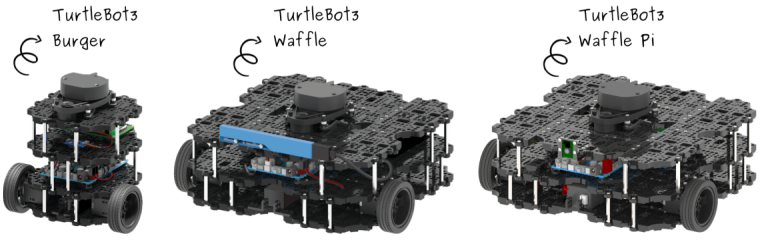
\includegraphics[width=1\textwidth]{tb3.png}
 \caption{TurtleBot3 Burger, Waffle and Waffle with Raspberry Pi (respectively)}
 \end{figure}
 
 \textbf{The following tutorial and demonstration focus on the TurtleBot3 Waffle}.
 
 \newpage

% ##### HARDWARE ASSEMBLE #####
 \section{Hardware Assemble} 

 The Waffle model consists of 3 different layers, each containing the required hardware. The first, or bottom, layer contains the wheels, it's motors and the battery. The second, or mid, layer accommodates the CPU, OpenCR (control board) and USB hub. The third, or top layer, containing the LIDAR sensor and 3D camera. Their exact positions may vary.
 
 The following steps briefly describe how to assemble the TurtleBot 3 Waffle. For more detailed information consult the official assemble tutorial provided by ROBOTIS
 
 \subsection{Layers}
 The first step is to assemble the layers. The bottom and mid ones assemble can be roughly visualized in the figure below. The top layer architecture is similar with a different orientation.  

 \begin{figure}[h]
 \centering
 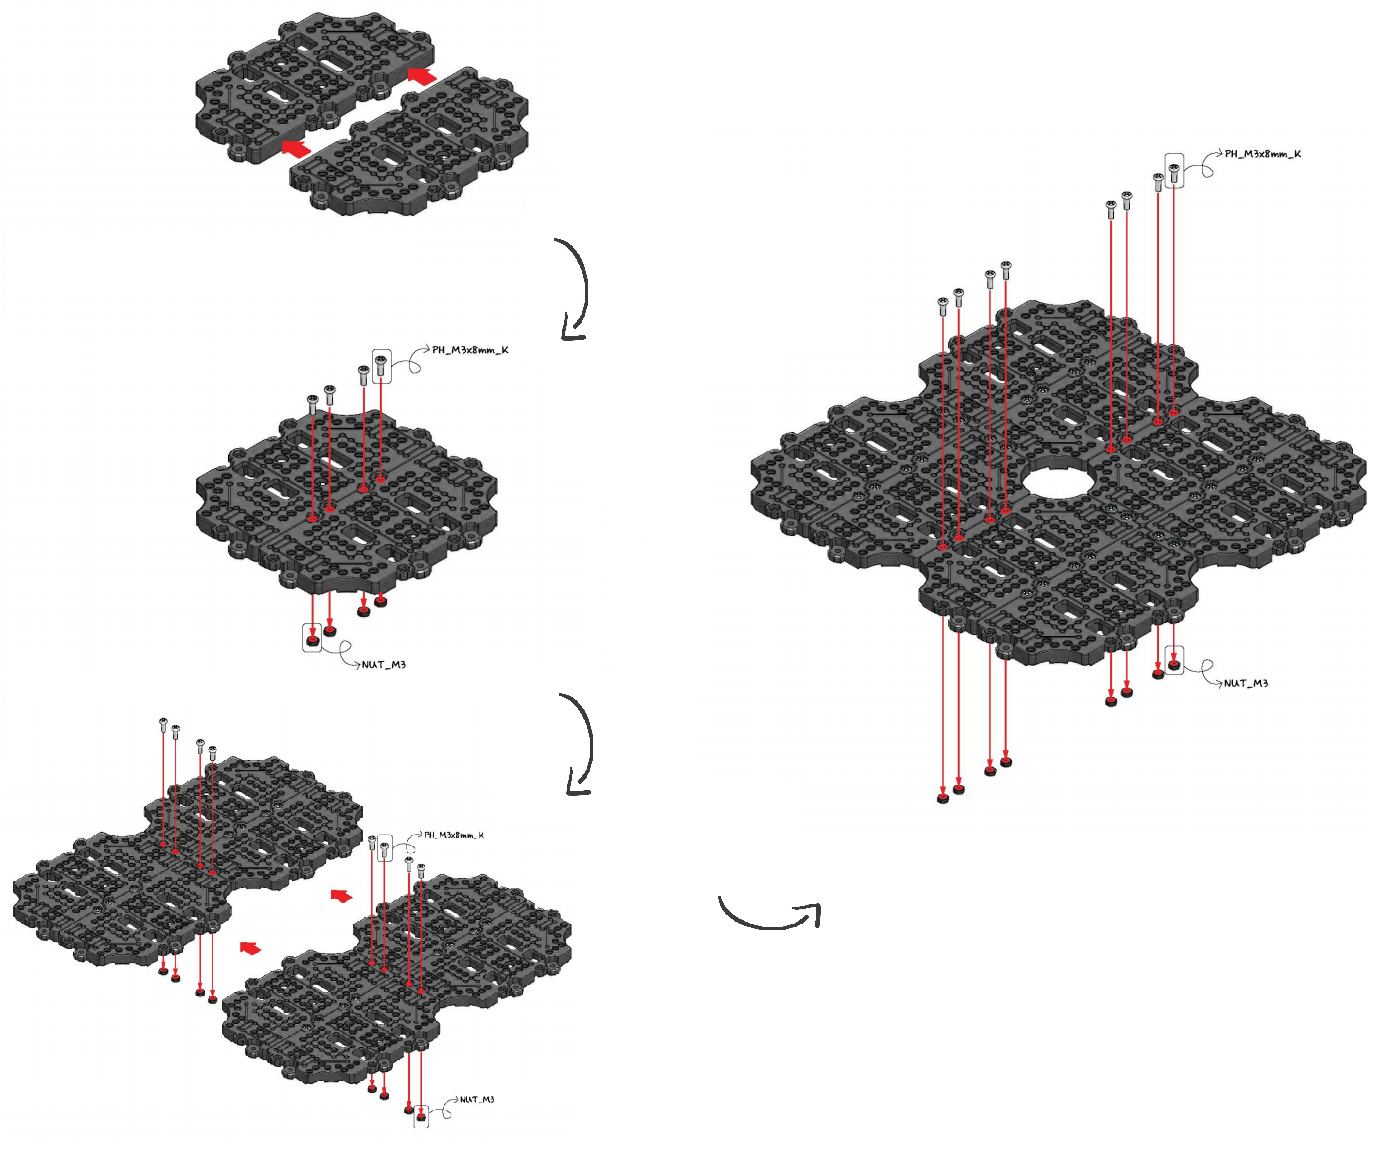
\includegraphics[width=1\textwidth]{step1.png}
 \caption{Bottom and Mid layer assemble}
 \end{figure}
 
 \subsection{Bottom Layer}
 
 The bottom layer accommodates the wheels, it's motors and the battery. 
 
  \begin{figure}[h]
 \centering
 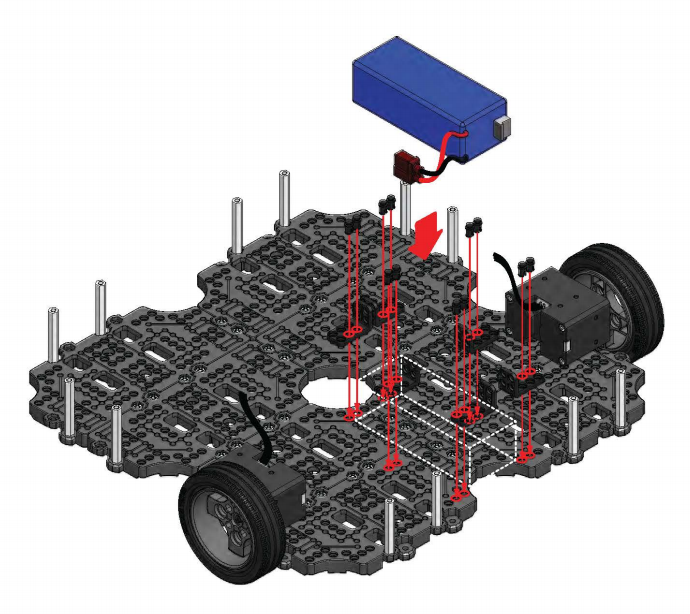
\includegraphics[width=0.4\textwidth]{layer1.png}
 \caption{Sketch representation of the bottom layer components assemble}
 \end{figure}
 
 \subsection{Top Layer}
 
 The top layer accomodates the LIDAR sensor and 3D camera.
 
    \begin{figure}[h]
 \centering
 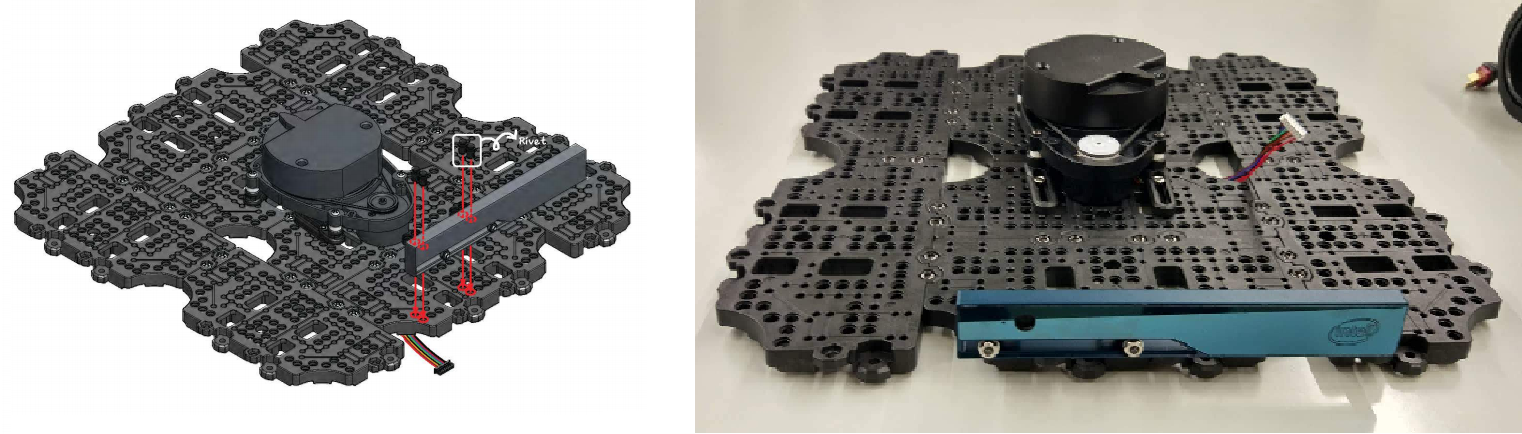
\includegraphics[width=1\textwidth,height=0.25\textheight]{toplayer.png}
 \caption{Sketch and real representation of the top layer components assemble}
 \end{figure}
 
 \newpage
 
 \subsection{Mid Layer}
 
 The mid layer accomodates the CPU, OpenCR (control board) and USB hub.
 
   \begin{figure}[h]
 \centering
 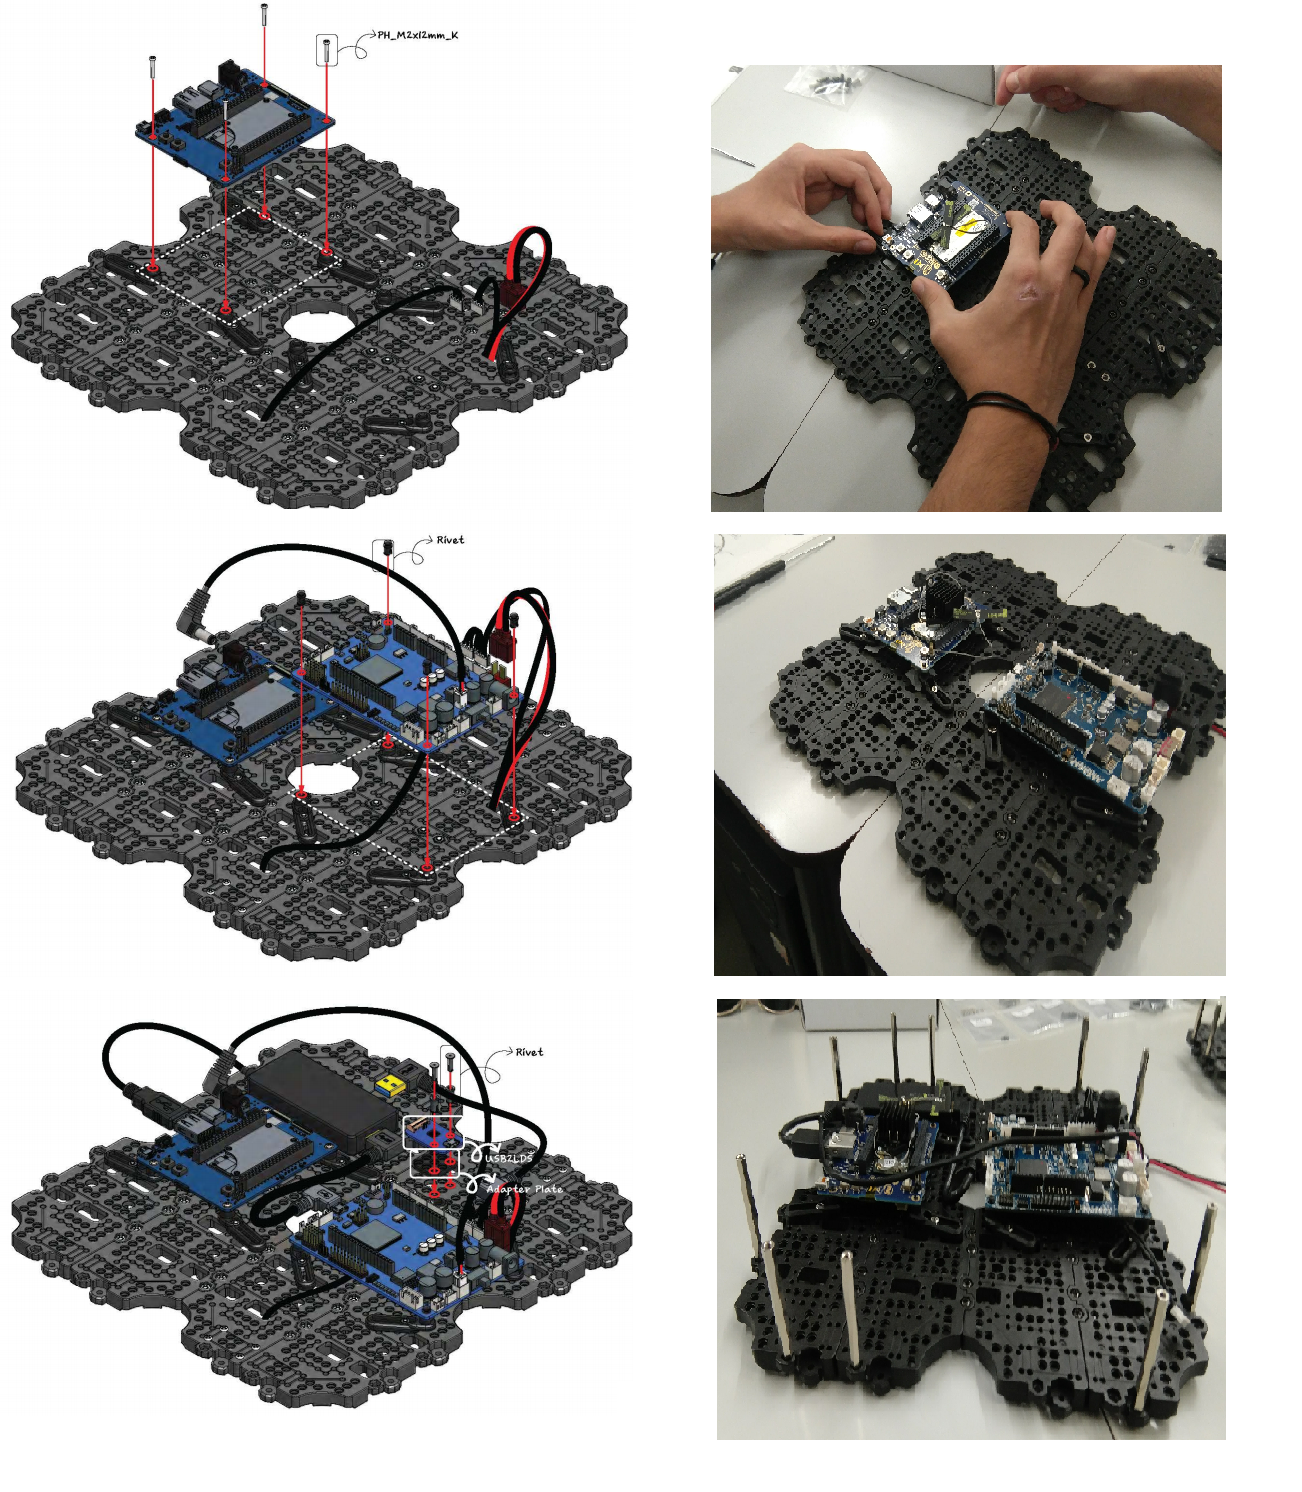
\includegraphics[width=1\textwidth]{midlayer.png}
 \caption{Sketch and real representation of the mid layer components assemble}
 \end{figure}
 
 \newpage
 
 \subsection{Layers Assemble}
 
 The final step is to join the layers together. 
 
    \begin{figure}[h]
 \centering
 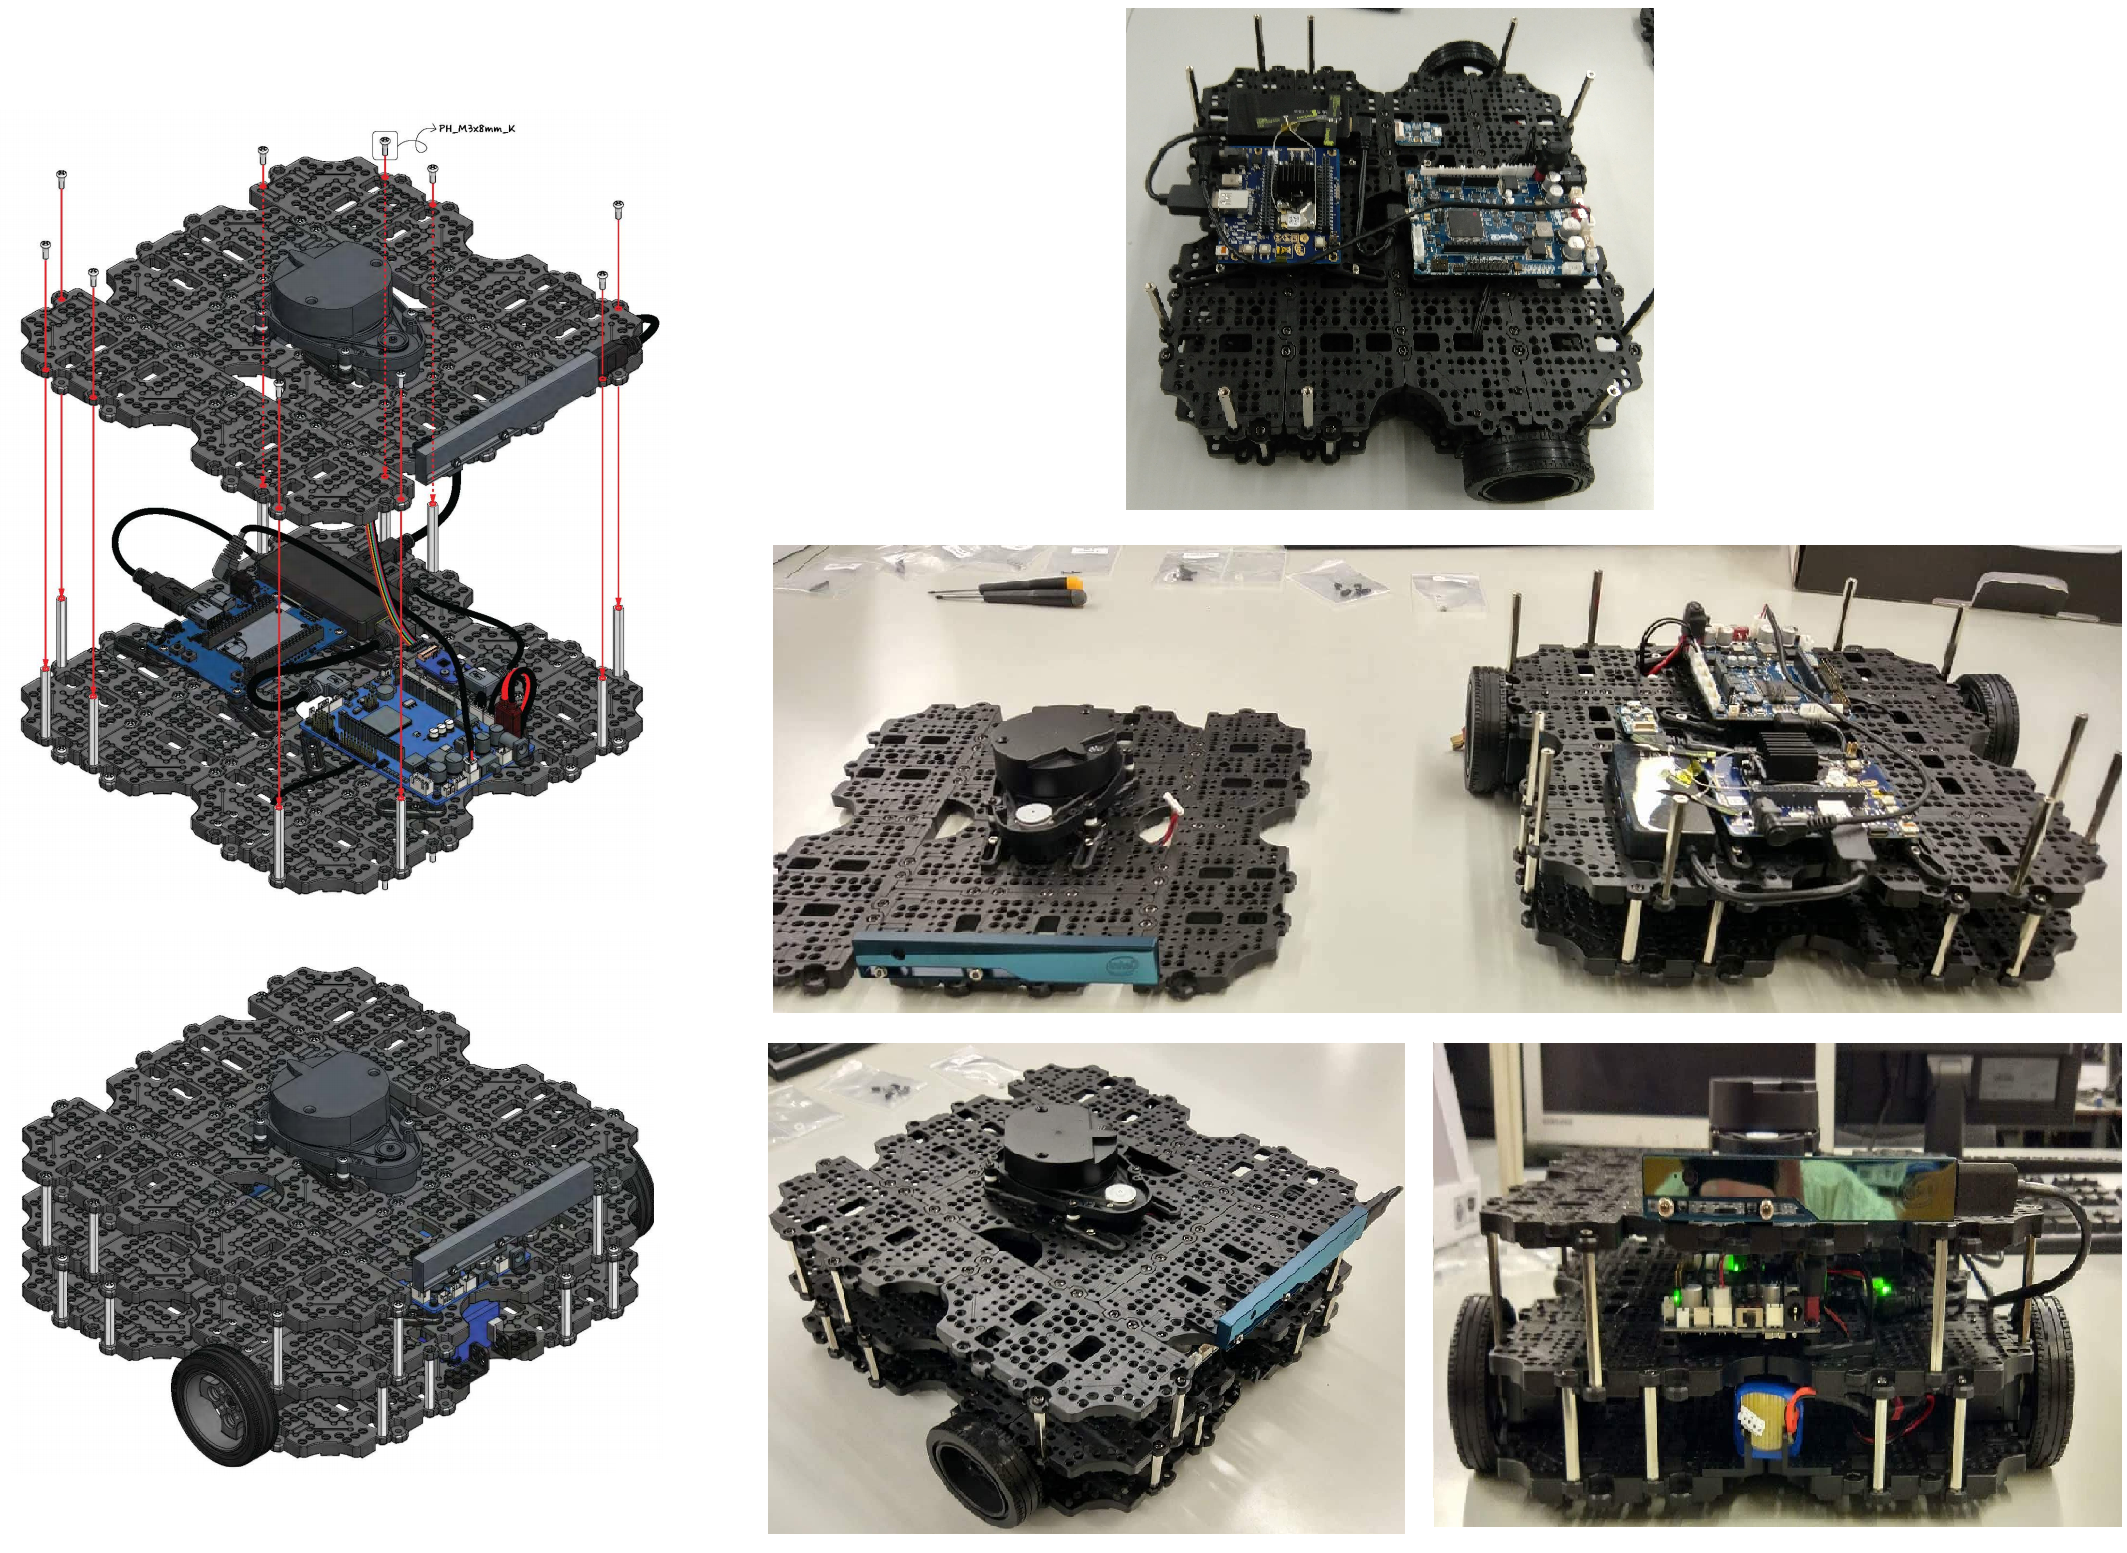
\includegraphics[width=1.1\textwidth,height=0.6\textheight]{finalasm.png}
 \caption{Sketch and real representation of the mid layer components assemble}
 \end{figure}
 
 \newpage
 
 % ##### SOFTWARE CONFIGURATION #####
 \section{Software Configuration}
 
 Upon assembling TurtleBot3, it is required to configure the software, both on the \textbf{robot} itself and on the \textbf{remote computer}. 
 
 It is not required but strongly suggested that both of the machines run the \textbf{Linux distribution, Ubuntu 16.04, and ROS Kinetic}s, plus the assigned \textbf{dependent packages for TurtleBot3 control}. The SSH connection setup enabled the communication between the robot and the remote PC. For more information on how to configure the environment refer to the TurtleBot3 ROBOTIS e-Manual.

\subsection{PC Setup}

The contents in this chapter corresponds to the Remote PC (your desktop or laptop PC) which will control TurtleBot3. Do \textbf{NOT} apply this instruction to your TurtleBot3.

\subsubsection{Install Ubuntu on Remote PC (Desktop or Laptop PC)}

Download Ubuntu 16.04 on the remote PC from https://www.ubuntu.com/download/desktop.

If you need more help for installing Ubuntu, check out the step-by-step guide at https://www.ubuntu.com/download/desktop/install-ubuntu-desktop.

\subsubsection{Install ROS on Remote PC}

In order to develop source code from the remote PC, please configure ROS environment after completing ROS installation.

The terminal application can be found with the Ubuntu search icon on the top left corner of the screen. Shortcut key for terminal is Ctrl-Alt-T.

Insert the following commands to the prompt of the terminal:

\begin{verbatim}
$ sudo apt-get update
$ sudo apt-get upgrade
$ wget https://raw.githubusercontent.com/ROBOTIS-GIT/\
robotis_tools/master/install_ros_kinetic.sh &&
chmod 755 ./install_ros_kinetic.sh &&
bash ./install_ros_kinetic.sh
\end{verbatim}

After install ROS, please reboot Remote PC.

\newpage

\subsubsection{Install Dependent packages on Remote PC}

The next step is to install dependent packages for TurtleBot3 control.

\begin{verbatim}
$ sudo apt-get install ros-kinetic-joy ros-kinetic-teleop-twist-joy\
ros-kinetic-teleop-twist-keyboard ros-kinetic-laser-proc\
ros-kinetic-rgbd-launch ros-kinetic-depthimage-to-laserscan\
ros-kinetic-rosserial-arduino ros-kinetic-rosserial-python\
ros-kinetic-rosserial-server ros-kinetic-rosserial-client\
ros-kinetic-rosserial-msgs ros-kinetic-amcl\
ros-kinetic-map-server ros-kinetic-move-base\
ros-kinetic-urdf ros-kinetic-xacro\
ros-kinetic-compressed-image-transport\
ros-kinetic-rqt-image-view ros-kinetic-gmapping\
ros-kinetic-navigation ros-kinetic-interactive-markers\
ros-kinetic-realsense-camera
\end{verbatim}

\subsubsection{Network Configuration}

ROS requires IP addresses in order to communicate between TurtleBot3 and the remote PC.

Enter the below command on the terminal window of the remote PC to find out the IP address of the remote PC.

\begin{verbatim}
$ ifconfig
\end{verbatim}

The output is similar to the image below and the IP of the remote PC is highlighted with the red rectangle.

\bigskip

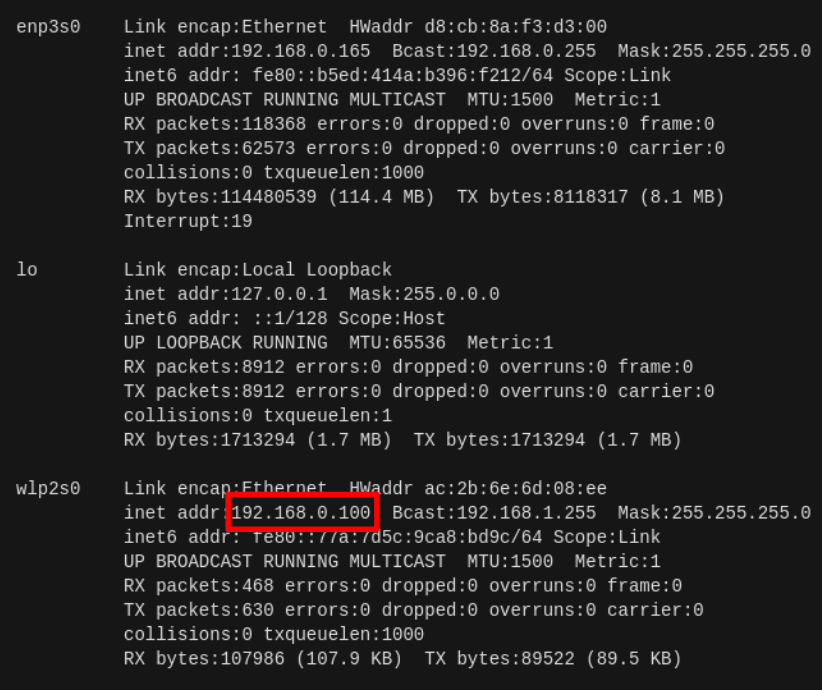
\includegraphics[width=0.7\textwidth]{network_configuration2}

\newpage

Now enter the command below.

\begin{verbatim}
$ nano ~/.bashrc
\end{verbatim}

Add the following text to the end of that file. Notice that you \textbf{have to change} the IP for the one you got before.

\begin{verbatim}
export ROS_MASTER_URI=htpp://192.168.0.100:11311
export ROS_HOSTNAME=192.168.0.100
\end{verbatim}

Then, source the bashrc with below command.

\begin{verbatim}
$ source ~/.bashrc
\end{verbatim}

\subsection{Turtlebot3 Setup}

The contents in this chapter corresponds to the Turtlebot3 configuration.

\subsubsection{Install Ubuntu}

In this section, the Alternative Ubuntu Desktop 16.04 LTS will be installed on Intel® Joule™.

\bigskip

\textbf{[Remote PC]} Download Ubuntu image Alternative Ubuntu 16.04 for Intel® Joule™ from http://people.canonical.com/~platform/snappy/tuchuck/desktop-final/tuchuck-xenial-desktop-iso-20170317-0.iso

\bigskip

\textbf{[Remote PC]} In order to make a bootable installation USB drive, please follow the Alternative install(Ubuntu Desktop 16.04 LTS) section from 

https://developer.ubuntu.com/core/get-started/intel-joule

\subsubsection{Install ROS on TurtleBot3}

The contents in this chapter corresponds to the Intel® Joule™ which will be the main computer of TurtleBot3 Waffle. Do NOT apply this instruction to your Remote PC (your desktop PC or laptop).

The terminal application can be found with the Ubuntu search icon on the top left corner of the screen. Shortcut key for terminal is Ctrl-Alt-T.

Insert the following commands to the prompt of the terminal:

\begin{verbatim}
$ sudo apt-get update
$ sudo apt-get upgrade
$ wget https://raw.githubusercontent.com/ROBOTIS-GIT/\
robotis_tools/master/install_ros_kinetic.sh &&
chmod 755 ./install_ros_kinetic.sh &&
bash ./install_ros_kinetic.sh
\end{verbatim}

After install ROS, please reboot Intel® Joule™.

\subsubsection{Install Dependent packages on TurtleBot3}

The next step is to install dependent packages for TurtleBot3 control.

\begin{verbatim}
$ sudo apt-get install ros-kinetic-rosserial-python ros-kinetic-tf
\end{verbatim}

\subsubsection{Network Configuration}

ROS requires IP addresses in order to communicate between TurtleBot3 and the remote PC.

Enter the below command on the terminal window of the remote PC to find out the IP address of the TurtleBot3.

\begin{verbatim}
$ ifconfig
\end{verbatim}

The output is similar to the image below and the IP of the TurtleBot3 is highlighted with the red rectangle.

\bigskip

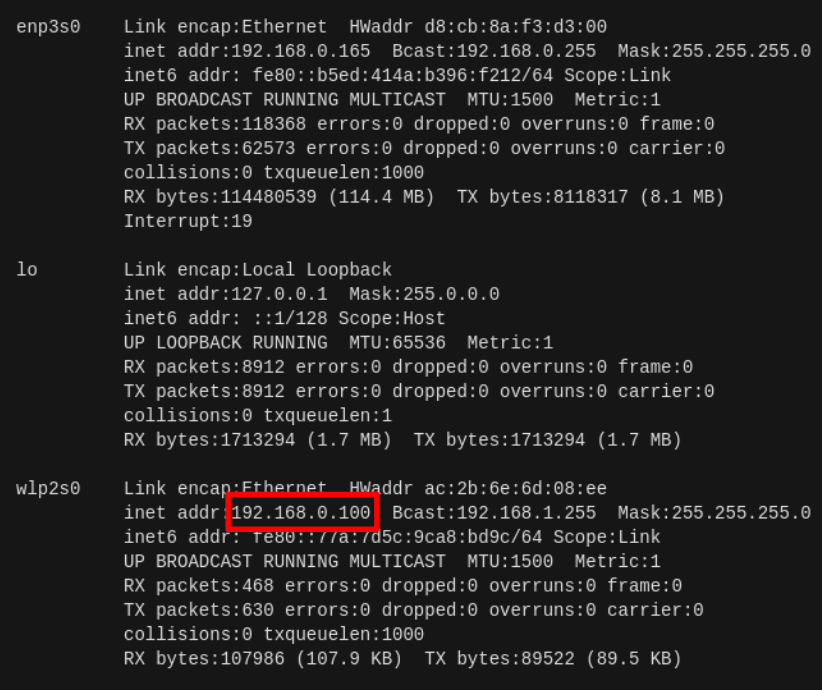
\includegraphics[width=0.7\textwidth]{network_configuration2}

\newpage

Now enter the command below.

\begin{verbatim}
$ nano ~/.bashrc
\end{verbatim}

Add the following text to the end of that file. Notice that you \textbf{have to change} the IP for the master uri for the one of the remote pc and the hostname for the one you got before.

\begin{verbatim}
export ROS_MASTER_URI=htpp://192.168.0.100:11311
export ROS_HOSTNAME=192.168.0.200
\end{verbatim}

Then, source the bashrc with below command.

\begin{verbatim}
$ source ~/.bashrc
\end{verbatim}

 \newpage
 
 \section{Demo}
 
Before start bringup TurtleBot3, We recommend you add export command to bashrc depend on your TurtleBot3.
 
Now enter the command below in the terminal of the TurtleBot3.

\begin{verbatim}
$ nano ~/.bashrc
\end{verbatim}

Add the following text to the end of that file.

\begin{verbatim}
export TURTLEBOT3_MODEL=waffle
\end{verbatim}

From the terminal of the remote PC run the following.

\begin{verbatim}
$ roscore
\end{verbatim}

Bring up basic packages to start TurtleBot3 applications. From the terminal of the TurtleBot3 run the following.

\begin{verbatim}
$ roslaunch turtlebot3_bringup turtlebot3_robot.launch
\end{verbatim}

\textbf{Tip} : If you want to launch Lidar sensor, Intel® RealSense™ R200 and core separately, please use below commands.

\begin{verbatim}
$ roslaunch turtlebot3_bringup turtlebot3_lidar.launch
$ roslaunch turtlebot3_bringup turtlebot3_realsense.launch
$ roslaunch turtlebot3_bringup turtlebot3_core.launch
\end{verbatim}

Now you just need to start implementing. Here is an example of a demo that makes the TurtleBot3 a follower using the LIDAR.

http://emanual.robotis.com/docs/en/platform/turtlebot3/applications/\#turtlebot-follower-demo
 
 \newpage
 
\section{Difficulties}
 
One of the main difficulties that you will have with TurtleBot3 is it's autonomy, our advice is that you simulate your implementation before hand and only after you are happy with the results of your simulation you should test the algorithm in the robot itself.

You should know and we can not stress this enough that the interaction between the sensors/actuators and the real environment is \textbf{VERY} different from what you will get in the simulator.

\end{document}
